\part{Monetisation}
\frame{\partpage}

\begin{frame}{Metrics of monetisation}
	\url{http://www.nicholaslovell.com}
	\url{https://www.appboy.com/blog/essential-mobile-app-metrics-formulas/}
	\url{https://www.slideshare.net/TomSente/game-monetization-analytics-how-to-use-your-game-metrics-effectively}
\end{frame}

\begin{frame}
	\begin{tikzpicture}[remember picture, overlay]
		\node[at=(current page.center)] {
			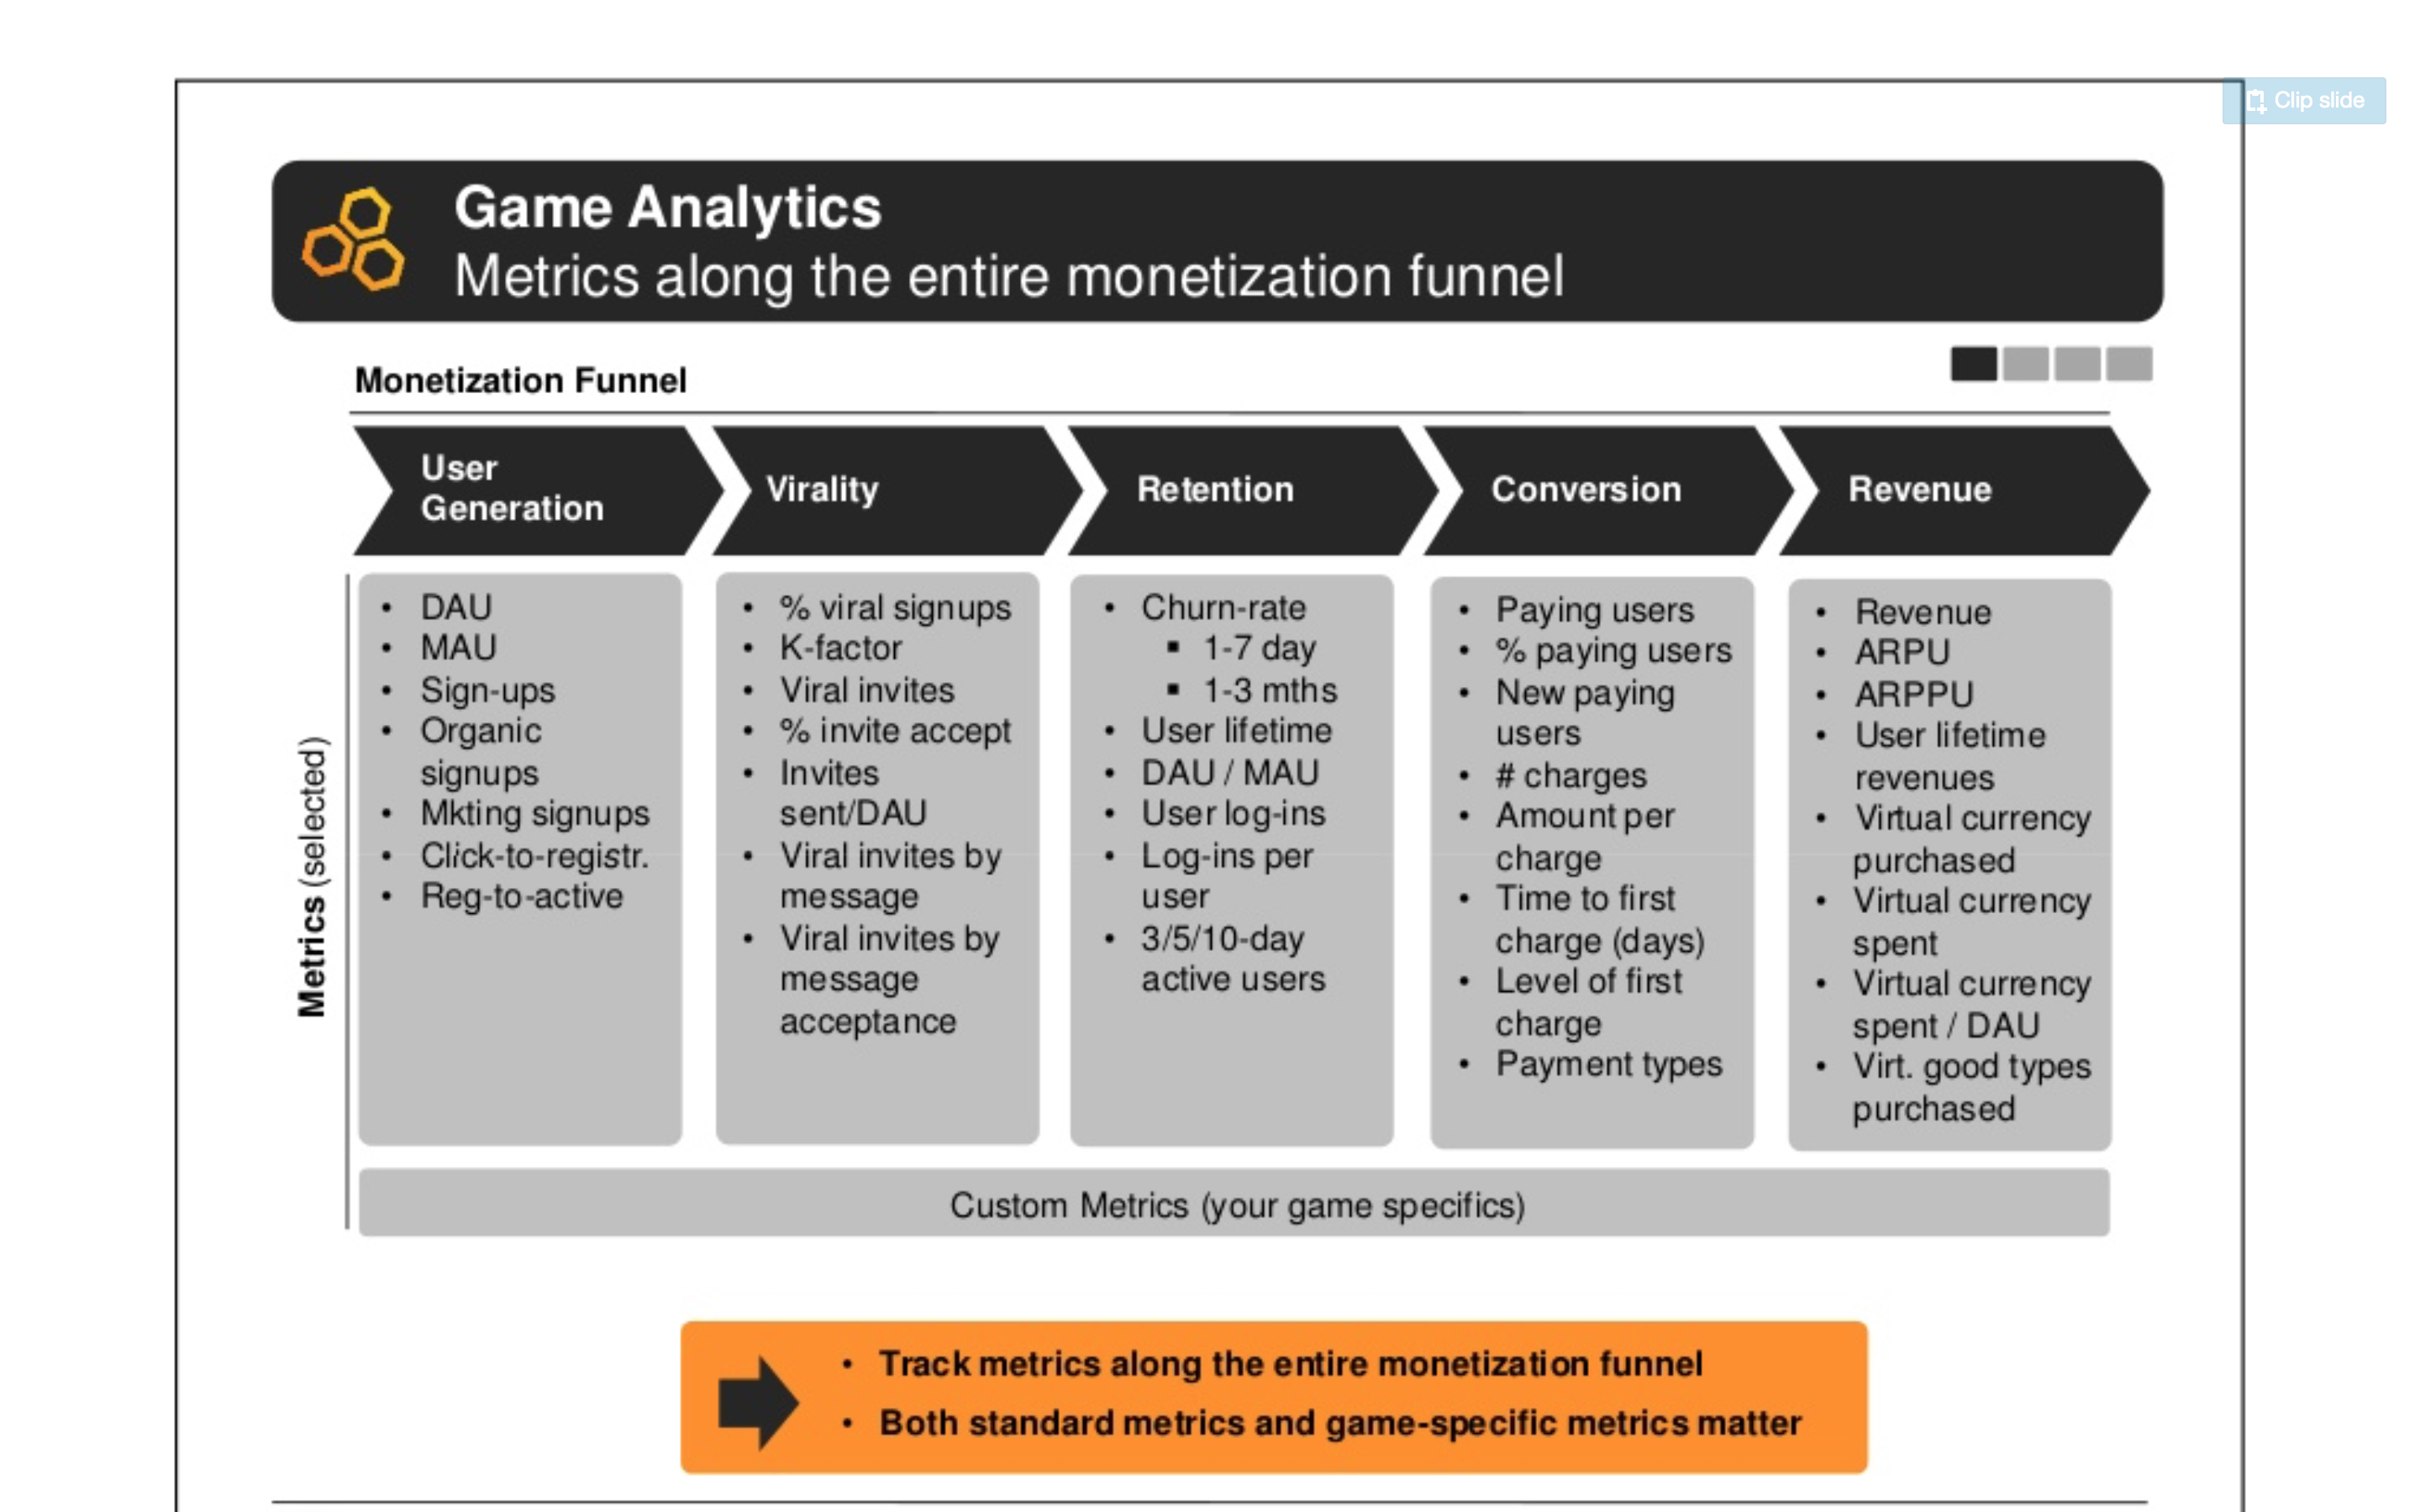
\includegraphics[width=\paperwidth]{f2p_metrics}
		};
	\end{tikzpicture}
\end{frame}

\begin{frame}{Metrics of monetisation}
	\begin{itemize}
		\pause\item A \textbf{metric} is any \textbf{measurable quantity}
		\pause\item Successful \textbf{free-to-play (F2P)} games (particularly on mobile) are driven by metrics
		\pause\item Metrics developed by \textbf{marketing}, \textbf{advertising},
			and \textbf{software-as-a-service (SaaS)} industries
		\pause\item The key to F2P success:
			$$ LTV > CPA $$
		\pause\item $LTV = $ life-time value 
			\begin{itemize}
				\pause\item How much each player spends over the entire time they continue playing the game
			\end{itemize}
		\pause\item $CPA = $ cost per acquisition
			\begin{itemize}
				\pause\item How much it costs to get each person playing the game (e.g.\ advertising)
			\end{itemize}
	\end{itemize}
\end{frame}

\begin{frame}{Stickiness}
	\begin{itemize}
		\pause\item $DAU$ = daily active users
		\pause\item $MAU$ = monthly active users
		\pause\item Stickiness $= \frac{DAU}{MAU}$
		\pause\item A ``sticky'' game is one that \textbf{keeps players coming back}
	\end{itemize}
\end{frame}

\begin{frame}{The curve}
	\begin{center}
		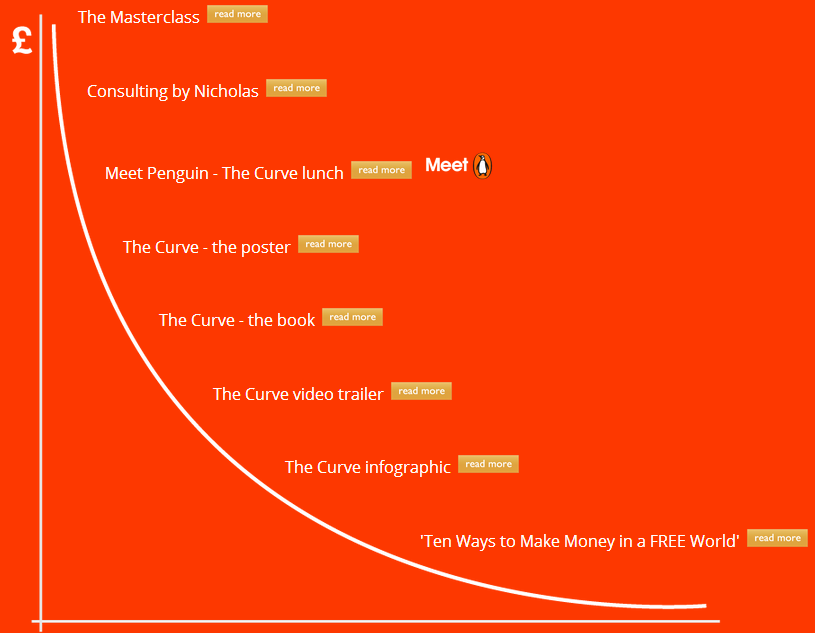
\includegraphics[height=0.8\textheight]{the_curve}
	\end{center}
\end{frame}

\begin{frame}{The curve}
	\begin{itemize}
		\pause\item Allow ``\textbf{superfans}'' (a.k.a.\ ``\textbf{whales}'') to spend large amounts
		\pause\item Allow ``\textbf{freeloaders}'' to spend little or nothing
			\begin{itemize}
				\pause\item ... but hopefully still generate word-of-mouth
			\end{itemize}
		\pause\item Not just for F2P --- also applies to reward tiers in crowdfunding
	\end{itemize}
\end{frame}
